% !TeX program = lualatex

\documentclass[a4paper]{report}

\usepackage{fontspec}
\setmainfont{Times New Roman}
\usepackage[
    top=3cm,
    bottom=3.5cm,
    left=3.5cm,
    right=2cm
]{geometry}
\usepackage{setspace}
\onehalfspacing
\usepackage{fancyhdr}
\usepackage{tocloft}
\usepackage{graphicx}
\usepackage{float}
\usepackage{hyperref}
\usepackage{amsmath}
\usepackage{amssymb}
\usepackage{array}
\usepackage{longtable}
\usepackage{booktabs}
\usepackage{titlesec}

\titleformat{\chapter}
  {\normalfont\huge\bfseries}
  {Chương \thechapter}
  {0.5em}
  {}
\titlespacing*{\chapter}{0pt}{-0.2in}{0.3in}

\renewcommand{\figurename}{Hình}
\renewcommand{\tablename}{Bảng}
\renewcommand{\contentsname}{Mục lục}
\renewcommand{\bibname}{Tài liệu tham khảo}
\renewcommand{\cftchapleader}{\cftdotfill{\cftdotsep}}
\renewcommand{\cftsecnumwidth}{3em}
\renewcommand{\cftsubsecnumwidth}{3em}

\pagestyle{fancy}
\fancyhf{}
\fancyfoot[C]{\thepage}
\renewcommand{\headrulewidth}{0pt}

\hypersetup{
    colorlinks=true,
    linkcolor=black,
    urlcolor=blue,
    citecolor=black
}

\begin{document}
\fontsize{13pt}{15.6pt}\selectfont
\pagenumbering{gobble}

\begin{titlepage}
    \centering
    \vspace*{1cm}

    {\Large\bfseries ĐẠI HỌC QUỐC GIA TP. HỒ CHÍ MINH}

    {\Large\bfseries TRƯỜNG ĐẠI HỌC CÔNG NGHỆ THÔNG TIN}

    {\Large\bfseries KHOA CÔNG NGHỆ PHẦN MỀM}

    \vspace{2.5cm}

    {\Large\bfseries BÁO CÁO ĐỒ ÁN}

    \vspace{1cm}

    {\LARGE\bfseries MEMESPLODING}

    \vspace{0.4cm}

    {\Large\bfseries TRÒ CHƠI BÀI MÈO NỔ TRỰC TUYẾN}

    \vspace{2.5cm}

    {\large\bfseries LỚP: CÔNG NGHỆ GAME ONLINE - SE315.Q21}

    \vspace{1cm}

    {\large\bfseries GIẢNG VIÊN HƯỚNG DẪN:}

    {\large ThS. Đặng Việt Dũng}

    \vspace{1cm}

    {\large\bfseries NHÓM 13:}

    {\large 23520819 - Quách Gia Kiệt}

    {\large 23520887 - Phạm Thành Long}

    {\large 23520790 - Võ An Khôi}

    {\large 23520905 - Võ Hồng Lương}

    \vfill

    {\large TP. HỒ CHÍ MINH, 2026}
\end{titlepage}

\chapter*{}
\begin{center}
    \Large\bfseries LỜI CẢM ƠN
\end{center}
\addcontentsline{toc}{chapter}{Lời cảm ơn}

Nhóm chúng em xin gửi lời cảm ơn chân thành đến ThS. Đặng Việt Dũng đã hỗ trợ,
góp ý và định hướng cho nhóm trong quá trình thực hiện đề tài Memesploding.
Những kiến thức và nhận xét của thầy đã giúp nhóm từng bước hoàn thiện sản phẩm,
từ việc phân tích yêu cầu, thiết kế hệ thống đến triển khai và kiểm thử.

Trong quá trình thực hiện, nhóm đã có cơ hội áp dụng kiến thức về phát triển phần
mềm, lập trình mạng, cơ sở dữ liệu và xây dựng trò chơi vào một sản phẩm hoàn
chỉnh. Do giới hạn về thời gian và kinh nghiệm, báo cáo vẫn có thể còn thiếu sót.
Nhóm mong nhận được thêm góp ý để tiếp tục cải thiện sản phẩm trong tương lai.

\vspace{1cm}
\begin{flushright}
    Nhóm sinh viên thực hiện\\
    Quách Gia Kiệt\\
    Phạm Thành Long\\
    Võ An Khôi\\
    Võ Hồng Lương
\end{flushright}

\newpage
\tableofcontents
\newpage

\chapter*{}
\begin{center}
    \Large\bfseries TÓM TẮT ĐỒ ÁN
\end{center}
\addcontentsline{toc}{chapter}{Tóm tắt đồ án}

\pagenumbering{arabic}
\setcounter{page}{1}
\pagestyle{fancy}

Memesploding là trò chơi bài trực tuyến nhiều người chơi, được xây dựng dựa trên
ý tưởng của trò chơi Mèo Nổ. Người chơi có thể tạo tài khoản, kết bạn, tạo hoặc
tham gia phòng, bắt đầu trận đấu và tương tác với nhau theo thời gian thực.

Hệ thống được tổ chức theo mô hình monorepo, gồm ứng dụng Unity dành cho người
chơi, API Server quản lý tài khoản và phòng chờ, Game Server xử lý luật chơi,
cùng các thành phần lưu trữ PostgreSQL và Redis. Trong trận đấu, máy chủ giữ
quyền quyết định trạng thái. Client chỉ gửi yêu cầu hành động, sau đó Game Server
kiểm tra tính hợp lệ, cập nhật trạng thái và gửi kết quả về cho các người chơi.

Đề tài đã triển khai các chức năng chính như xác thực, quản lý hồ sơ, bạn bè,
thông báo, phòng chơi, ghép trận, lịch sử trận đấu và gameplay thời gian thực.
Hệ thống cũng hỗ trợ khôi phục trạng thái khi người chơi mất kết nối trong một
khoảng thời gian cho phép.

\chapter{Mở đầu}

\section{Lý do chọn đề tài}

Các trò chơi trực tuyến nhiều người chơi là một bài toán phù hợp để áp dụng nhiều
kiến thức của ngành công nghệ phần mềm. Một sản phẩm như vậy không chỉ cần giao
diện dễ sử dụng mà còn phải giải quyết vấn đề đồng bộ dữ liệu, xử lý kết nối mạng,
quản lý trạng thái và bảo đảm luật chơi được thực hiện công bằng.

Nhóm lựa chọn phát triển Memesploding nhằm xây dựng một trò chơi có cách chơi
gần gũi, vui nhộn và có thể chơi cùng bạn bè. Đề tài đồng thời tạo điều kiện để
nhóm thực hành xây dựng một hệ thống hoàn chỉnh gồm client, backend, cơ sở dữ
liệu và giao tiếp thời gian thực.

\section{Mục tiêu}

Mục tiêu của đề tài là xây dựng một trò chơi bài trực tuyến có các khả năng sau:

\begin{itemize}
    \item Cho phép người dùng đăng ký, đăng nhập và quản lý hồ sơ.
    \item Hỗ trợ kết bạn, thông báo và xem bảng xếp hạng.
    \item Cho phép tạo phòng, tham gia phòng và ghép trận nhanh.
    \item Vận hành một trận đấu Mèo Nổ theo thời gian thực.
    \item Kiểm tra luật chơi ở phía máy chủ để hạn chế gian lận.
    \item Hỗ trợ người chơi kết nối lại và nhận đúng trạng thái hiện tại.
    \item Lưu kết quả và cho phép xem lịch sử trận đấu.
\end{itemize}

\section{Đối tượng sử dụng}

Đối tượng sử dụng của Memesploding là người chơi yêu thích thể loại game bài
nhẹ nhàng, có tính tương tác và có thể chơi cùng nhóm bạn. Ứng dụng hướng đến
các phiên chơi ngắn, dễ tiếp cận và không yêu cầu người chơi phải có nhiều kinh
nghiệm trước đó.

\section{Phạm vi đề tài}

Phiên bản hiện tại tập trung vào bộ bài gốc và các cơ chế cốt lõi như rút bài,
đánh bài hành động, phản ứng Nope, xử lý Exploding Kitten và sử dụng Defuse.
Mỗi trận hỗ trợ nhiều người chơi trong cùng một phòng. Hệ thống được thiết kế
cho giai đoạn thử nghiệm nội bộ và ưu tiên tính ổn định của gameplay.

Các chức năng mở rộng như khán giả, trò chuyện trong trận, nhiều bộ bài mở rộng
và vận hành Game Server trên nhiều máy chưa phải trọng tâm của phiên bản này.

\chapter{Cơ sở lý thuyết và công nghệ}

\section{Mô hình client--server}

Trong mô hình client--server, client chịu trách nhiệm nhận thao tác và hiển thị
kết quả cho người dùng. Server tiếp nhận yêu cầu, xử lý nghiệp vụ và quản lý dữ
liệu dùng chung. Mô hình này phù hợp với game trực tuyến vì trạng thái trận đấu
không nên do từng client tự quyết định.

Memesploding sử dụng Unity làm game client. Backend được tách thành API Server
và Game Server. Cách tách này giúp phần quản lý tài khoản, phòng chờ và dữ liệu
lâu dài không bị trộn với phần xử lý gameplay có nhiều yêu cầu về thời gian thực.

\section{ASP.NET Core}

ASP.NET Core là nền tảng được sử dụng để xây dựng hai máy chủ của hệ thống.
API Server cung cấp các REST API cho xác thực, người dùng, bạn bè, phòng chơi,
thông báo và lịch sử trận đấu. Game Server tiếp nhận các lệnh gameplay và điều
phối trạng thái của từng trận.

Hệ thống sử dụng cơ chế Dependency Injection của ASP.NET Core để đăng ký và
quản lý các service. Các tác vụ nền được triển khai bằng Hosted Service, phục vụ
việc nhận sự kiện, cập nhật runtime, kiểm tra timeout và xử lý kết nối lại.

\section{Unity}

Unity được sử dụng để xây dựng giao diện và phần tương tác của trò chơi. Client
gồm các thành phần quản lý scene, phòng chơi, gameplay, âm thanh, API và kết nối
WebSocket. Dữ liệu lá bài được tổ chức bằng ScriptableObject để thuận tiện cho
việc quản lý nội dung và hiển thị.

Client không tự quyết định kết quả của hành động. Khi người chơi đánh hoặc rút
bài, Unity gửi command đến Game Server và cập nhật giao diện dựa trên event hoặc
snapshot nhận lại.

\section{SignalR và giao tiếp thời gian thực}

SignalR hỗ trợ giao tiếp hai chiều giữa server và client. Memesploding sử dụng
hai endpoint SignalR:

\begin{itemize}
    \item API WebSocket phục vụ sự kiện phòng, lời mời và trạng thái người dùng.
    \item Game WebSocket phục vụ command và event trong trận đấu.
\end{itemize}

Các message được chuẩn hóa theo cấu trúc gồm tên sự kiện, dữ liệu và thời điểm
gửi. Trạng thái trận có số phiên bản tăng dần để client phát hiện dữ liệu mới và
yêu cầu snapshot khi cần.

\section{PostgreSQL và Entity Framework Core}

PostgreSQL lưu dữ liệu cần tồn tại lâu dài như người dùng, hồ sơ, quan hệ bạn bè,
bộ bài, lá bài, thông báo và lịch sử trận đấu. Entity Framework Core được sử dụng
để ánh xạ entity, truy vấn dữ liệu và quản lý migration.

\section{Redis}

Redis lưu các dữ liệu có vòng đời ngắn hoặc cần truy cập nhanh, gồm trạng thái
phòng, sự hiện diện của người chơi, snapshot trận đấu và các kênh sự kiện giữa
API Server với Game Server. Redis Pub/Sub giúp hai máy chủ trao đổi sự kiện mà
không phụ thuộc trực tiếp vào nhau.

\section{JSON Web Token}

JSON Web Token được dùng để xác thực request đến API và kết nối SignalR. Sau
khi đăng nhập, client nhận access token và sử dụng token này trong các lần giao
tiếp tiếp theo. Khi bắt đầu trận, hệ thống cấp game ticket chứa thông tin phòng,
người chơi và trận đấu để Game Server kiểm tra kết nối.

\chapter{Phân tích và thiết kế hệ thống}

\section{Yêu cầu chức năng}

Các nhóm chức năng chính của hệ thống được trình bày trong Bảng
\ref{tab:functions}.

\begin{longtable}{p{0.25\textwidth} p{0.63\textwidth}}
    \caption{Các nhóm chức năng chính}
    \label{tab:functions}                                                        \\
    \toprule
    \textbf{Nhóm chức năng} & \textbf{Mô tả}                                     \\
    \midrule
    \endfirsthead
    \toprule
    \textbf{Nhóm chức năng} & \textbf{Mô tả}                                     \\
    \midrule
    \endhead
    Tài khoản               &
    Đăng nhập khách, đăng ký và đăng nhập bằng email, đăng nhập Google, làm mới
    token, đăng xuất và khôi phục mật khẩu.                                      \\
    Hồ sơ                   &
    Xem và cập nhật hồ sơ, xem thống kê, tìm người dùng và bảng xếp hạng.        \\
    Bạn bè                  &
    Gửi, chấp nhận hoặc từ chối lời mời kết bạn và xóa bạn bè.                   \\
    Phòng chơi              &
    Tạo phòng, tham gia, rời phòng, cập nhật cấu hình, sẵn sàng và bắt đầu trận. \\
    Ghép trận               &
    Tự động tìm hoặc tạo phòng phù hợp cho người chơi.                           \\
    Gameplay                &
    Chia bài, rút bài, đánh bài, xử lý hiệu ứng, Nope, Defuse, loại người chơi
    và xác định người thắng.                                                     \\
    Thông báo               &
    Nhận, đọc, xóa thông báo và theo dõi số thông báo chưa đọc.                  \\
    Lịch sử                 &
    Lưu kết quả, xem lịch sử và thông tin chi tiết của trận đấu.                 \\
    \bottomrule
\end{longtable}

\section{Yêu cầu phi chức năng}

Hệ thống cần bảo đảm trạng thái giữa các người chơi được đồng bộ, thao tác trong
trận có độ trễ thấp và dữ liệu riêng như bài trên tay không bị gửi cho người khác.
Game Server phải kiểm tra mọi command trước khi thay đổi trạng thái. Hệ thống
cũng cần có khả năng phục hồi khi người chơi mất kết nối tạm thời.

Mã nguồn được chia thành các module có trách nhiệm rõ ràng để dễ bảo trì. Các
contract dùng chung giữa API Server và Game Server được đặt trong project Shared
nhằm hạn chế sai lệch dữ liệu khi phát triển.

\section{Kiến trúc tổng thể}

Hệ thống gồm các thành phần chính:

\begin{itemize}
    \item \textbf{Unity Client}: hiển thị giao diện, nhận thao tác và giao tiếp với server.
    \item \textbf{API Server}: quản lý tài khoản, hồ sơ, bạn bè, phòng chờ và lịch sử.
    \item \textbf{Game Server}: quản lý runtime và thực thi luật của trận đấu.
    \item \textbf{PostgreSQL}: lưu dữ liệu lâu dài.
    \item \textbf{Redis}: lưu trạng thái tạm thời, snapshot và truyền sự kiện.
\end{itemize}

API Server sở hữu trạng thái phòng trước trận, gồm các trạng thái chờ và chuẩn
bị bắt đầu. Khi trận được tạo thành công, quyền xử lý gameplay được chuyển cho
Game Server. Sau khi trận kết thúc, Game Server gửi kết quả về API Server để lưu
và đưa phòng trở lại trạng thái chờ.

\section{Thiết kế API Server}

API Server được tổ chức theo các lớp controller, service, data, hub, middleware
và worker. Controller nhận HTTP request và chuyển xử lý cho service. Service thực
hiện nghiệp vụ và truy cập PostgreSQL hoặc Redis. Middleware xử lý lỗi và kiểm
tra token. App Hub phát các sự kiện thời gian thực liên quan đến người dùng và
phòng chơi.

Các nhóm REST API chính gồm authentication, users, friends, rooms, matchmaking,
notifications, matches và card sets. Dữ liệu trả về được chuẩn hóa thành response
đơn, response danh sách hoặc response lỗi.

\section{Thiết kế Game Server}

Game Server áp dụng nguyên tắc server authoritative. Mỗi phòng đang chơi có một
\texttt{MatchRuntime} riêng. Mọi command của trận được đưa vào hàng đợi và xử lý
tuần tự. Thiết kế này tránh trường hợp hai hành động cùng thay đổi một trạng thái
vào cùng thời điểm.

Luồng xử lý command gồm:

\begin{enumerate}
    \item Game Hub nhận command từ client.
    \item Game Command Dispatcher xác định handler phù hợp.
    \item Handler kiểm tra người chơi, lượt và trạng thái hiện tại.
    \item Match Runtime cập nhật trạng thái và tạo event.
    \item Event được gửi đến các client trong phòng.
    \item Snapshot mới được lưu vào Redis tại các thời điểm cần thiết.
\end{enumerate}

Các engine và effect handler trong tầng Domain xử lý lượt chơi, cửa sổ phản ứng,
vụ nổ và hiệu ứng của từng loại lá bài. Tầng Infrastructure đảm nhiệm snapshot,
event stream, thời gian và giao tiếp với API Server.

\section{Thiết kế dữ liệu}

PostgreSQL chứa các bảng chính:

\begin{itemize}
    \item \texttt{users}: thông tin định danh và xác thực.
    \item \texttt{profiles}: biệt danh, ảnh đại diện, cấp độ và điểm xếp hạng.
    \item \texttt{friendships}: quan hệ và trạng thái lời mời kết bạn.
    \item \texttt{card\_sets}, \texttt{cards}: thông tin bộ bài và lá bài.
    \item \texttt{matches}: thông tin tổng quát của trận đã kết thúc.
    \item \texttt{match\_participants}: kết quả của từng người chơi.
    \item \texttt{notifications}: thông báo gửi đến người dùng.
\end{itemize}

Redis lưu room metadata, danh sách thành viên, trạng thái sẵn sàng, thông tin
người dùng đang ở phòng, snapshot gameplay và các channel tích hợp.

\section{Thiết kế khôi phục kết nối}

Khi mất kết nối, Game Server đánh dấu người chơi là disconnected nhưng chưa loại
ngay khỏi trận. Snapshot hiện tại được giữ trong Redis. Nếu người chơi kết nối
lại trong thời gian cho phép, client gửi yêu cầu reconnect và nhận snapshot đã
được lọc theo quyền xem. Unity dùng snapshot này để dựng lại bài trên tay, lượt,
người chơi và các hiệu ứng đang chờ.

\chapter{Kết quả triển khai}

\section{Chức năng tài khoản và hồ sơ}

Hệ thống hỗ trợ tài khoản khách, email và Google. Sau khi xác thực, người chơi có
thể xem hoặc cập nhật biệt danh, ảnh đại diện và phần giới thiệu. Các thông tin
thống kê như cấp độ, điểm, số trận và số trận thắng được hiển thị trong hồ sơ và
bảng xếp hạng.

\section{Chức năng bạn bè và thông báo}

Người chơi có thể tìm kiếm người dùng, gửi lời mời kết bạn và xử lý các lời mời
nhận được. Sự kiện liên quan đến bạn bè và phòng được cập nhật qua API WebSocket.
Hệ thống thông báo cho phép đánh dấu đã đọc hoặc xóa thông báo.

\section{Phòng chơi và ghép trận}

Người chơi có thể tạo phòng công khai, tham gia bằng mã phòng hoặc sử dụng ghép
trận nhanh. Trong phòng chờ, thành viên theo dõi danh sách người chơi và trạng
thái sẵn sàng. Chủ phòng có quyền cập nhật một số cấu hình và bắt đầu trận khi
các điều kiện đã được đáp ứng.

\begin{figure}[H]
    \centering
    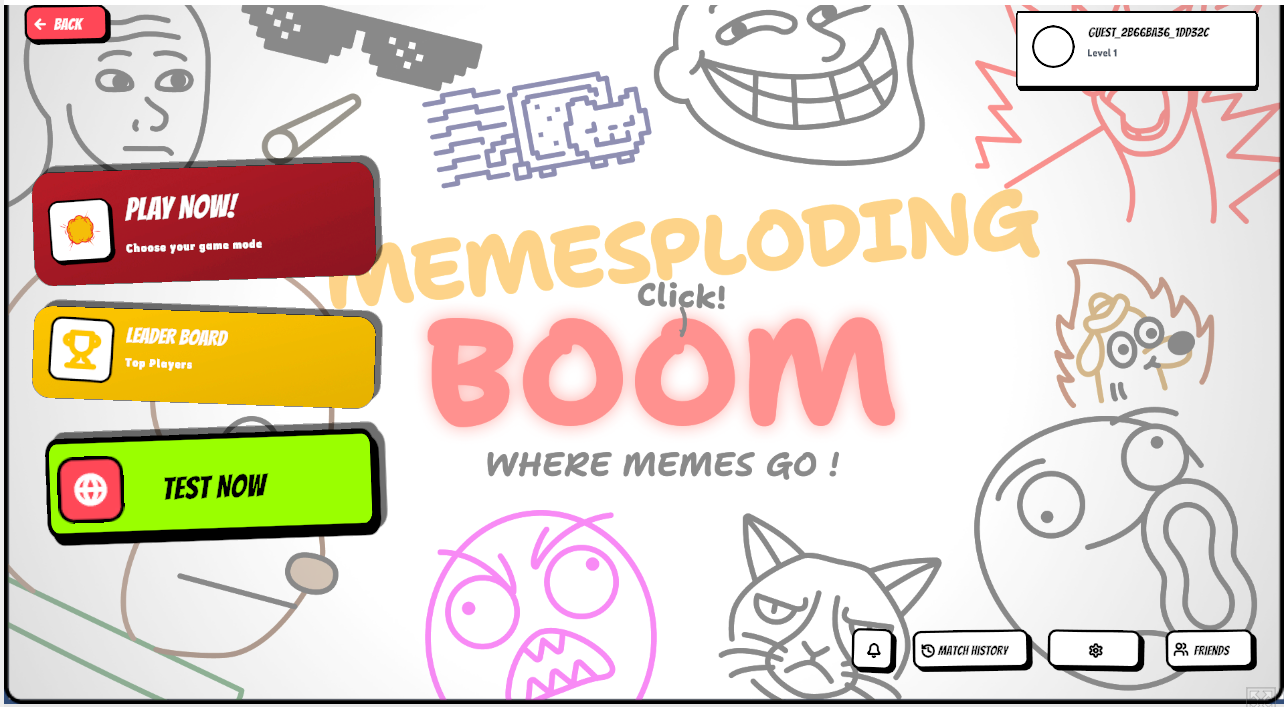
\includegraphics[width=0.95\textwidth]{lobby.png}
    \caption{Giao diện sảnh chính của trò chơi}
    \label{fig:lobby}
\end{figure}

\section{Gameplay thời gian thực}

Khi trận bắt đầu, Game Server tạo bộ bài, chia bài và chọn người đi đầu. Trong
mỗi lượt, người chơi có thể đánh bài hoặc rút bài. Các hành động cần phản ứng sẽ
mở một khoảng thời gian để người khác sử dụng Nope. Khi rút Exploding Kitten,
người chơi phải dùng Defuse nếu có; nếu không sẽ bị loại khỏi trận.

Giao diện gameplay hiển thị bài trên tay, bộ bài rút, lượt hiện tại, thời gian còn
lại và trạng thái của các đối thủ. Client chỉ cho phép gửi những thao tác phù hợp
với trạng thái đang hiển thị, trong khi Game Server tiếp tục kiểm tra lại để bảo
đảm tính hợp lệ.

\begin{figure}[H]
    \centering
    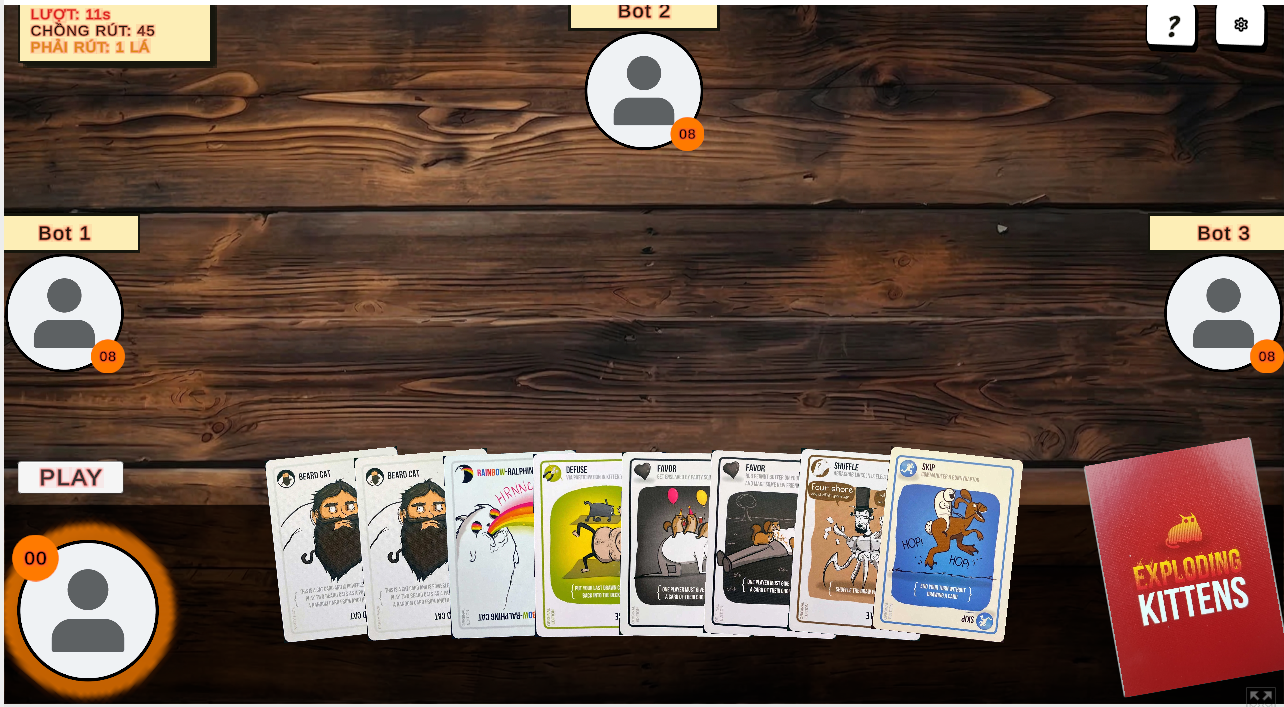
\includegraphics[width=0.95\textwidth]{gameplay.png}
    \caption{Giao diện gameplay trong trận đấu}
    \label{fig:gameplay}
\end{figure}

\section{Lịch sử và bảng xếp hạng}

Sau khi trận kết thúc, kết quả được gửi về API Server để lưu vào PostgreSQL.
Người chơi có thể xem lịch sử trận, thứ hạng, điểm thay đổi và thông tin các
người tham gia. Bảng xếp hạng sắp xếp người chơi theo điểm hiện tại.

\section{Kiểm thử}

Dự án có các bài kiểm thử đơn vị cho Game Server, tập trung vào luật chơi, hiệu
ứng lá bài và các chuyển đổi trạng thái. Ngoài ra, nhóm sử dụng HTTP test và web
test harness để kiểm tra REST API, SignalR, luồng phòng và gameplay nhiều người
chơi.

Các tình huống cần kiểm tra gồm command không đúng lượt, đánh lá bài không có
trong tay, chuỗi Nope, hết thời gian phản ứng, xử lý Defuse, mất kết nối và kết
nối lại. Việc sử dụng random seed cố định trong một số trường hợp giúp tái hiện
trận đấu và so sánh kết quả.

\section{Đánh giá kết quả}

\subsection{Ưu điểm}

\begin{itemize}
    \item Hệ thống có đầy đủ các thành phần từ giao diện đến backend và lưu trữ.
    \item API Server và Game Server có ranh giới trách nhiệm tương đối rõ ràng.
    \item Gameplay được kiểm tra ở server, giúp hạn chế gian lận từ client.
    \item SignalR đáp ứng tốt nhu cầu cập nhật trạng thái theo thời gian thực.
    \item Snapshot và state version hỗ trợ khôi phục sau khi mất kết nối.
    \item Kiến trúc cho phép bổ sung lá bài và hiệu ứng mới theo từng handler.
\end{itemize}

\subsection{Hạn chế}

\begin{itemize}
    \item Phiên bản hiện tại chủ yếu tập trung vào bộ bài gốc.
    \item Khả năng chịu tải lớn và vận hành nhiều Game Server chưa được hoàn thiện.
    \item Một số luồng giao diện và thông báo lỗi còn có thể được cải thiện.
    \item Hệ thống kiểm thử tích hợp và kiểm thử tải cần được mở rộng thêm.
    \item Các tính năng xã hội trong trận như trò chuyện và khán giả chưa có.
\end{itemize}

\chapter{Kết luận}

Đề tài đã xây dựng được Memesploding, một trò chơi bài trực tuyến gồm Unity
client, API Server, Game Server, PostgreSQL và Redis. Sản phẩm đáp ứng các luồng
cơ bản từ đăng nhập, quản lý hồ sơ, tạo phòng đến chơi và lưu kết quả trận đấu.

Thông qua đề tài, nhóm đã áp dụng được kiến thức về kiến trúc client--server,
REST API, WebSocket, cơ sở dữ liệu và quản lý trạng thái thời gian thực. Việc tách
API Server khỏi Game Server giúp hệ thống rõ ràng hơn về trách nhiệm và tạo nền
tảng để tiếp tục mở rộng.

Sản phẩm vẫn còn các giới hạn về quy mô vận hành, nội dung bộ bài và độ hoàn
thiện của trải nghiệm người dùng. Tuy nhiên, phiên bản hiện tại đã chứng minh
được luồng kỹ thuật chính và có thể dùng làm nền tảng cho các giai đoạn tiếp theo.

\chapter{Hướng phát triển}

Trong tương lai, nhóm có thể phát triển thêm các nội dung sau:

\begin{itemize}
    \item Bổ sung các bộ bài mở rộng và thêm nhiều hiệu ứng mới.
    \item Hoàn thiện giao diện, hoạt ảnh, âm thanh và hướng dẫn người chơi.
    \item Thêm trò chuyện, biểu cảm, khán giả và hệ thống mời bạn vào trận.
    \item Cải thiện matchmaking dựa trên điểm xếp hạng và khu vực.
    \item Tổ chức giải đấu, nhiệm vụ hằng ngày và phần thưởng.
    \item Mở rộng Game Server theo nhiều instance và bổ sung cơ chế định tuyến.
    \item Tăng độ phủ kiểm thử tự động, kiểm thử tải và giám sát hệ thống.
    \item Phát hành trên nhiều nền tảng và tối ưu trải nghiệm trên thiết bị di động.
\end{itemize}

\addcontentsline{toc}{chapter}{Tài liệu tham khảo}
\begin{thebibliography}{9}
    \bibitem{aspnet}
    Microsoft,
    \textit{ASP.NET Core Documentation}.
    \url{https://learn.microsoft.com/aspnet/core/}

    \bibitem{signalr}
    Microsoft,
    \textit{ASP.NET Core SignalR Documentation}.
    \url{https://learn.microsoft.com/aspnet/core/signalr/}

    \bibitem{efcore}
    Microsoft,
    \textit{Entity Framework Core Documentation}.
    \url{https://learn.microsoft.com/ef/core/}

    \bibitem{unity}
    Unity Technologies,
    \textit{Unity Documentation}.
    \url{https://docs.unity3d.com/}

    \bibitem{postgresql}
    PostgreSQL Global Development Group,
    \textit{PostgreSQL Documentation}.
    \url{https://www.postgresql.org/docs/}

    \bibitem{redis}
    Redis,
    \textit{Redis Documentation}.
    \url{https://redis.io/docs/}
\end{thebibliography}

\end{document}
